\documentclass[11pt]{article}

\usepackage[margin=1in]{geometry}
\usepackage{amsmath, amssymb, amsthm}
\usepackage{booktabs}
\usepackage{graphicx}
\usepackage{microtype}
\usepackage{natbib}
\usepackage[hidelinks]{hyperref}

\newcommand{\R}{\mathbb{R}}
\newcommand{\Sig}{\Sigma}
\newcommand{\F}{\mathcal{F}}
\newcommand{\B}{\mathcal{B}}
\newcommand{\Aset}{\mathcal{A}}
\newcommand{\Sset}{\mathcal{S}}
\newcommand{\trans}{^{\top}}
\newcommand{\lb}{\ell}
\newcommand{\ub}{u}

\theoremstyle{plain}
\newtheorem{theorem}{Theorem}
\newtheorem{proposition}{Proposition}
\newtheorem{lemma}{Lemma}
\theoremstyle{definition}
\newtheorem{remark}{Remark}

\title{Following the Solution:\\
Parametric Active-Set Homotopies in Statistics, Optimization, and Finance}

\author{[Authors]\thanks{Perspective draft for \emph{Statistical Science}. We build
on, and dedicate this account to, the work of Harry Markowitz (1927--2023).}}
\date{Draft, \today}

\begin{document}
\maketitle

\begin{abstract}
Many methods across statistics, optimization, and finance return not a single
solution but a \emph{path} of solutions as one scalar parameter is swept: the LASSO
follows the $\ell_1$-regularised coefficients along the penalty; the support-vector
machine follows the dual variables along the cost; explicit model predictive control
precomputes the control law along the state; and Markowitz's Critical Line Algorithm,
older than all of them, follows the optimal portfolio along risk aversion. We argue,
and prove on the cleanest pair, that these are one device. Our contribution is an
exact identity, not an analogy: with the covariance taken to be a Gram matrix, the
constrained mean--variance frontier and the constrained LASSO path are the
\emph{same} piecewise-linear curve, with breakpoints in bijection, and this survives
arbitrary linear equality and inequality constraints, well beyond the unconstrained
correspondence and the single gross-exposure case known since
\citet{brodie2009}. Around the theorem we organise the family by the small list of
features that actually distinguish its members (whether the active set is imposed by
constraints or induced by a penalty, whether it only grows or also shrinks, and what
structure the quadratic form carries), recount the history in which the device was
invented in the 1950s, forgotten by statistics, and rediscovered around 2000, and
collect the questions the unified view makes precise, chiefly the gap between the
linear path length seen in practice and the exponential one possible in theory.
\end{abstract}

\section{Introduction}

This is a paper about one algorithm that four fields invented separately and never
fully recognised as shared. The algorithm follows the optimiser of a parametrised
strictly convex quadratic as a single scalar moves; the solution traces a
piecewise-linear curve, and an active set is all the state needed to trace it
exactly. In statistics it is least angle regression and the LASSO homotopy
\citep{tibshirani1996, osborne2000, efron2004}; in machine learning the regularization
path of the support vector machine \citep{hastie2004svm} and the elastic net and
generalized lasso \citep{zou2005, tibshirani2011}; in control the explicit linear
quadratic regulator computed by multi-parametric quadratic programming
\citep{bemporad2002, tondel2003}; and in finance, decades earlier, Markowitz's
Critical Line Algorithm for the efficient frontier \citep{markowitz1956,
markowitz1959}.

We make three claims, and we lead with them rather than with the survey. First
(Section~\ref{sec:identity}), the connection between the two most dissimilar-looking
members, a portfolio optimizer and a sparse regression, is an \emph{exact identity}:
under one substitution the constrained Markowitz frontier and the constrained LASSO
path are the same curve, breakpoint for breakpoint, and the identity holds under
arbitrary linear constraints. We state this as a theorem and prove it. Second
(Section~\ref{sec:taxonomy}), once the identity is in hand, the entire family is
organised by a short list of distinguishing features, and the apparent diversity of
the methods collapses onto that list. Third (Sections~\ref{sec:tour}--\ref{sec:comp}),
the unification is not only conceptual: a single implementation, accessing its
quadratic form as an operator, traces every instance, and structured forms (factor
models, kernels) are the lever that carries the sixty-year-old algorithm to modern
scale.

The synthesis is, in places, a synthesis of known parts, and we are explicit about
which (Section~\ref{sec:history} and throughout). What is new is the exact
general-constraint identity and the organisation it makes possible; what is old, and
worth retelling, is that statistics spent the 2000s rediscovering a device finance
and optimization had in the 1950s.

\section{The common scheme}
\label{sec:scheme}

Fix a strictly convex quadratic whose linear part carries a scalar $\lambda$,
minimised over a polyhedron:
\begin{equation}
\label{eq:pqp}
x(\lambda) = \arg\min_{x \in \R^n}\ \tfrac12\, x\trans H x - \lambda\, d\trans x
\quad\text{s.t.}\quad A x = b,\ G x \le h,\ \lb \le x \le \ub , \qquad H \succ 0 .
\end{equation}
A polyhedral \emph{penalty} such as $\lambda\|x\|_1$ fits the same template through its
subgradient, as Section~\ref{sec:identity} makes explicit. This is a one-parameter
parametric quadratic program; its solution map has the structure that is the whole
story.

\begin{lemma}[Affine segments]
\label{lem:affine}
On any maximal interval of $\lambda$ on which the active set (the equalities, the
active inequality rows, and the variables at a box bound) is constant, the optimiser
of \eqref{eq:pqp} is affine in $\lambda$,
\begin{equation}
\label{eq:affine}
x(\lambda) = \alpha + \lambda\,\beta ,
\end{equation}
for constant $\alpha,\beta$ determined by $H$ and the active constraint normals.
\end{lemma}

\begin{proof}
With the active set fixed, the KKT conditions of \eqref{eq:pqp} are a square linear
system in $x$ and the active multipliers whose coefficient matrix depends only on $H$
and the active normals, and whose right-hand side is $\lambda d$ plus constants from
the fixed bound values and active right-hand sides. The system is nonsingular because
$H\succ 0$ and the active normals are linearly independent at a vertex of the
parametric program, so its solution is an affine function of the only $\lambda$-dependent
term, $\lambda d$. Restricting to $x$ gives \eqref{eq:affine}.
\end{proof}

The intervals partition the $\lambda$-axis at \emph{breakpoints} where the active set
must change; \citet{rosset2007} gave the clean sufficient condition (a quadratic loss
with a polyhedral penalty or constraint), and in control the same fact is the
piecewise-affinity of the mpQP solution over \emph{critical regions}
\citep{bemporad2002}. Continuity of $x(\lambda)$ across breakpoints (from strict
convexity) lets a \emph{homotopy} recover the whole path: from a vertex with known
active set, follow \eqref{eq:affine} to the first event, update the active set by that
one event, repeat. Each step is one solve against the active block of $H$ bordered by
the active normals. Event selection, ``the smallest positive step to the next
breakpoint,'' is the simplex method's ratio test, and it inherits the simplex
method's degeneracy hazard and its remedy: a lowest-index (Bland) tie-break that makes
the walk deterministic. We call \eqref{eq:pqp}, \eqref{eq:affine}, and this homotopy
the \emph{common scheme}.

\paragraph{$H$ is an operator, not a matrix.}
It is worth stating at the outset what the homotopy actually asks of $H$, because it is
much less than ``a stored $n\times n$ matrix.'' Inspecting the step of
Lemma~\ref{lem:affine}, the quadratic form enters only through three linear actions:
a matrix--vector product $v\mapsto Hv$, a solve $Hv = r$ restricted to the active
block, and the cross product coupling active and inactive coordinates. Anything that
supplies those three actions can play the role of $H$; the matrix is never needed
explicitly. This is not a fussy implementation point but the source of the scheme's
reach. A factor risk model $\Sig = \operatorname{diag}(\delta) + U\Lambda U\trans$
with $k\ll n$ factors, or a kernel Gram matrix $H = \kappa(X,X)$, supplies the three
actions in $O(nk)$ or through the kernel trick \emph{without ever forming the
$n\times n$ object}, the factor case through the Woodbury identity. Reading $H$ as an
operator rather than a matrix is therefore what keeps the common scheme, and the
identity of Section~\ref{sec:identity}, generic across dense covariances, factor
models, and kernels alike; we return to it in Section~\ref{sec:comp}.

\section{The exact identity}
\label{sec:identity}

We now show that the two most dissimilar members of the family are, under one
substitution, the same instance of the common scheme, and that the identity is robust
to general constraints.

\paragraph{The two programs.}
For weights $w\in\R^n$, expected returns $\mu$, and covariance $\Sig\succ 0$, the
gross-exposure-constrained mean--variance program is
\begin{equation}
\label{eq:mark}
\text{M}_c:\quad \min_{w}\ \tfrac12\, w\trans \Sig\, w - \mu\trans w
\quad\text{s.t.}\quad \|w\|_1 \le c,\ \ A w = b,\ \ G w \le h .
\end{equation}
For a response $y\in\R^m$ and design $X\in\R^{m\times n}$, the constrained LASSO is
\begin{equation}
\label{eq:lasso}
\text{L}_\lambda:\quad \min_{\beta}\ \tfrac12\,\|y - X\beta\|_2^2 + \lambda\,\|\beta\|_1
\quad\text{s.t.}\quad A\beta = b,\ \ G\beta \le h .
\end{equation}

\begin{theorem}[CLA--LASSO identity under general constraints]
\label{thm:identity}
Suppose $\Sig = X\trans X$ and $\mu = X\trans y$. Then for every $\lambda\ge 0$ there is
a $c(\lambda)=\|\beta(\lambda)\|_1$ such that $\mathrm{M}_{c(\lambda)}$ and
$\mathrm{L}_\lambda$ have the same minimiser, and $c(\lambda)$ is nonincreasing. The
solution path of $\mathrm{M}_c$ as $c$ varies and the regularization path of
$\mathrm{L}_\lambda$ as $\lambda$ varies are therefore the \emph{same}
piecewise-linear curve in $\R^n$, with their breakpoints in bijection. The same
active-set homotopy traces both.
\end{theorem}

\begin{proof}
Completing the square, $\tfrac12\|y-Xw\|_2^2 = \tfrac12 w\trans (X\trans X) w -
(X\trans y)\trans w + \tfrac12\|y\|_2^2$. With $\Sig=X\trans X$ and $\mu=X\trans y$ the
objective of $\mathrm{M}_c$ equals $\tfrac12\|y-Xw\|_2^2$ up to the additive constant
$\tfrac12\|y\|_2^2$, which does not affect the minimiser. Hence, under the same linear
constraints $Aw=b,\ Gw\le h$, $\mathrm{M}_c$ is exactly the constrained least-squares
problem $\min_w \tfrac12\|y-Xw\|_2^2$ subject to $\|w\|_1\le c$ and those constraints.
Its Lagrangian relaxation of the single constraint $\|w\|_1\le c$ is
$\min_w \tfrac12\|y-Xw\|_2^2 + \lambda\|w\|_1$ subject to $Aw=b,\ Gw\le h$, i.e.\
$\mathrm{L}_\lambda$. Because the objective is convex and $\|\cdot\|_1$ is convex,
strong duality holds for the norm-ball constraint, and the constrained and penalised
forms have identical solution sets as $c$ and $\lambda$ range over $[0,\infty)$, with
$c(\lambda)=\|\beta(\lambda)\|_1$ the active constraint level at the dual value
$\lambda$; $c(\lambda)$ is nonincreasing because larger penalties shrink $\|\beta\|_1$.
Both objectives are quadratic and both feasible sets are polyhedral, so by
Lemma~\ref{lem:affine} each path is piecewise linear; since the two programs share a
minimiser at every parameter value, the two paths are the same set of points, and the
breakpoints (the parameter values at which the active set changes) are in bijection
under $\lambda\mapsto c(\lambda)$. Tracing either by the homotopy of
Section~\ref{sec:scheme} visits the same vertices in the same order.
\end{proof}

\begin{remark}
The unconstrained ($A,G$ absent) case is the textbook LARS/LASSO correspondence; the
single gross-exposure case with a budget is \citet{brodie2009}. The content of
Theorem~\ref{thm:identity} is that arbitrary linear equalities and inequalities pass
through unchanged: an active inequality row $g_i\trans x = h_i$ enters the reduced KKT
system exactly as an equality, by stacking $C=[\,A;\,G_{\Sset}\,]$ over the active rows
$\Sset$ and replacing $A$ with $C$ in the segment solve of Lemma~\ref{lem:affine}.
Statistics rarely has an \emph{exact} constrained LASSO path; coordinate descent and
proximal methods approximate it on a grid, and LARS omits the constraints. The
portfolio side supplies it for free.
\end{remark}

\paragraph{Bound versus penalty.}
The identity has a structural reading. In $\mathrm{M}_c$ the sparsity is governed by
an \emph{explicit} constraint, the gross-exposure ball; in $\mathrm{L}_\lambda$ it is
\emph{induced} by a penalty through its subgradient. The next proposition records
exactly when the two descriptions coincide and when the explicit one becomes vacuous.

\begin{proposition}[The gross-exposure hinge]
\label{prop:hinge}
For a long-only, fully invested portfolio ($w\ge 0$, $\mathbf{1}\trans w = 1$) the
gross-exposure constraint is vacuous, since $\|w\|_1 = \mathbf{1}\trans w = 1$ for all
feasible $w$; the constraint $\|w\|_1\le c$ binds only for $c\ge 1$, where it is
inactive. The long-only mean--variance problem is therefore a \emph{non-negative}
LASSO with the equality $\mathbf{1}\trans\beta=1$, and it traces a frontier rather than
a sparsity path. Short positions admitted under a binding cap $\|w\|_1\le c$ with
$c>1$ make the constraint active, and then $\mathrm{M}_c$ and $\mathrm{L}_\lambda$
coincide as in Theorem~\ref{thm:identity}.
\end{proposition}

\begin{proof}
Immediate from $\|w\|_1=\sum_i |w_i| = \sum_i w_i = \mathbf{1}\trans w$ when $w\ge0$,
so the budget fixes $\|w\|_1=1$ and $\|w\|_1\le c$ cannot bind for $c\ge1$; for $c<1$
the long-only budget is infeasible. With short positions $\|w\|_1>\mathbf{1}\trans w$
in general, and the cap binds for $c$ below the unconstrained $\|w\|_1$.
\end{proof}

Figure~\ref{fig:both} shows the shared object: a single piecewise-linear coefficient
path, traced here as a LASSO, whose breakpoints carry two vocabularies at once.

\begin{figure}[t]
\centering
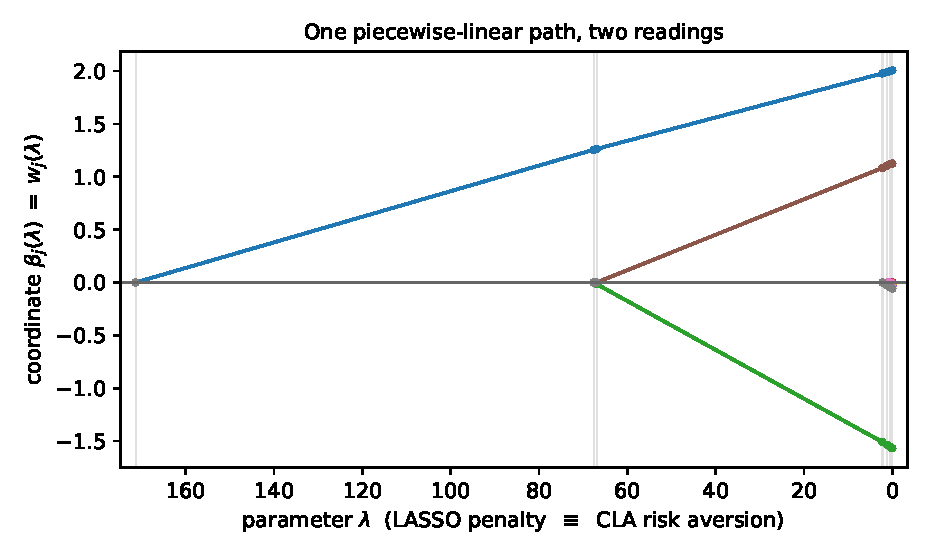
\includegraphics[width=0.74\textwidth]{path_both_sides.pdf}
\caption{One piecewise-linear path, two readings. The coordinate paths
$\beta_j(\lambda)=w_j(\lambda)$ of a small problem traced by the shared homotopy
(\texttt{cvxcla}). Each breakpoint (vertical guide) is simultaneously a LASSO event
and a Critical Line Algorithm event: a coordinate \emph{entering} the support when
its correlation reaches $\lambda$ is, on the portfolio side, a blocked multiplier
changing sign; a coordinate \emph{leaving} when its coefficient reaches zero is a free
weight reaching a bound. The curve is identical; only the names differ.}
\label{fig:both}
\end{figure}

\section{Shared scaffolding, particular features}
\label{sec:taxonomy}

With the identity in hand, the family is organised not by field of origin but by a
short list of features, against a large shared core. The core is all of
Section~\ref{sec:scheme}: the parametric QP, the affine segment, the homotopy, the
simplex-inherited anti-cycling. Four features distinguish the members.

\emph{Imposed versus induced active sets.} Constraints (the CLA, constrained
regression) impose faces; penalties (the LASSO, generalized lasso, SVM path) induce
them through a subgradient. Theorem~\ref{thm:identity} and
Proposition~\ref{prop:hinge} show the two are interconvertible, with the
gross-exposure ball the hinge, but their computational ergonomics differ, which is
why each field built its own version.

\emph{Monotone versus non-monotone active sets.} Forward selection and forward LARS
only \emph{add} variables; the LASSO modification and the CLA throughout both add and
drop, since coefficients can return to zero and weights can leave and re-enter their
bounds as $\lambda$ moves. The CLA corresponds to the full LASSO homotopy, not to
forward LARS.

\emph{The structure of $H$.} The scheme touches the data only through the quadratic
form: a covariance in finance, a Gram matrix in regression, a kernel matrix in the SVM
path. What $H$ is fixes both interpretation and cost, and, crucially, the homotopy
never needs it explicitly (Section~\ref{sec:comp}).

\emph{Degeneracy.} Ties and near-rank-deficiency are the recurring practical hazard;
the inherited Bland rule guarantees determinism but, as in the simplex method, does not
fully tame the adversarial worst case (Section~\ref{sec:length}).

\section{A tour of the instances}
\label{sec:tour}

Read through the taxonomy, the instances are short to describe. The \textbf{LASSO}
\citep{tibshirani1996, efron2004} is induced, non-monotone, $H=X\trans X$. The
\textbf{SVM regularization path} \citep{hastie2004svm} is induced, non-monotone, $H$ a
kernel matrix; the \textbf{elastic net} \citep{zou2005} adds a ridge, sending
$H\to X\trans X+\eta I$; the \textbf{generalized lasso} \citep{tibshirani2011} traces a
piecewise-linear \emph{dual} path for penalties $\lambda\|D\beta\|_1$ (fused lasso,
trend filtering, graph penalties). The \textbf{Critical Line Algorithm}
\citep{markowitz1956, markowitz1959} is imposed, non-monotone, $H=\Sig$; it is the
oldest instance by four decades. \textbf{Explicit MPC} \citep{bemporad2002, tondel2003}
is the multidimensional cousin, with a vector parameter and a polyhedral partition into
critical regions in place of the interval of breakpoints. Each is the common scheme with
$(H,d)$ and a face-mechanism filled in; none requires new machinery.

\section{History}
\label{sec:history}

\subsection{The Critical Line Algorithm}
\label{sec:cla-history}

The active-set treatment of the parametric quadratic program is a creation of the
1950s, and the Critical Line Algorithm is its earliest fully worked instance.
\citet{markowitz1952} posed mean--variance selection; recognising that the efficient
set is obtained by solving a quadratic program \emph{parametrically} in the
risk--return trade-off, \citet{markowitz1956} gave the Critical Line Algorithm,
announced in its title as ``the optimization of a quadratic function subject to linear
constraints,'' and developed it in full in the 1959 monograph \citep{markowitz1959}.
The method is exactly the homotopy of Section~\ref{sec:scheme}: trace the critical
line, changing the status of one asset at each turning point. It is contemporary with,
and independent of, the general active-set quadratic-programming theory of the same
years, notably \citet{wolfe1959}, who in \emph{Econometrica} adapted the simplex
method to quadratic programming and fixed the ratio-test-and-pivot lineage the homotopy
still rides.

Two threads then ran for half a century. On the modelling side, \citet{sharpe1963}, at
Markowitz's suggestion, introduced the single-index model, writing the covariance as a
diagonal matrix plus a single rank-one term to tame the estimation and computational
burden of a dense $\Sig$. Modern multi-factor risk models generalise this
diagonal-plus-low-rank form, and it is precisely the structure the operator reading of
$H$ (Sections~\ref{sec:scheme} and~\ref{sec:comp}) exploits: the covariance the
classical CLA treats as a dense matrix is, in practice, almost never dense. On the
algorithmic side, the CLA was re-derived, refined, and scaled across decades:
\citet{perold1984} for large-scale portfolio optimization, then \citet{stein2008} and
\citet{hirschberger2010} for active-set and large-universe variants,
\citet{niedermayer2010} for a careful fast implementation, \citet{markowitz2000} for
the canonical textbook description and reference code, and \citet{bailey2013} for a
widely used open-source version; \citet{markowitz2021} gives a recent step-by-step
account extending the method to mean--semivariance. Throughout, the algorithm was
presented as a portfolio method, and its membership in a wider homotopy family was not
the question being asked.

\subsection{And how statistics came to it independently}
\label{sec:stats-history}

Statistics arrived at the same device around forty years later, by a different door,
and at first without reference to any of this. \citet{osborne2000} gave a homotopy for
the LASSO of \citet{tibshirani1996}; \citet{efron2004} gave least angle regression and
made the piecewise-linear path famous; \citet{hastie2004svm} extended it to the support
vector machine, and \citet{rosset2007} characterised, within statistics, exactly when
such a path is piecewise linear, recovering for the field the criterion the
parametric-programming literature had long had. The methods were presented as native to
regularised estimation.

The bridge back was late and partial. \citet{brodie2009} observed that a
gross-exposure-constrained Markowitz problem \emph{is} a LASSO, the special case of
Theorem~\ref{thm:identity} without general constraints. Even so, the observation
travelled as a curiosity rather than as the statement that two large algorithmic
literatures describe one method. That is the gap this paper closes: not a new
algorithm, but the recognition, made exact and general, that the algorithm was never
four.

\section{Computation: one engine, many problems}
\label{sec:comp}

The unification has a software corollary. Because every step of the homotopy accesses
$H$ only through a matrix--vector product, a solve against the active block, and an
active-to-inactive cross product, one implementation serves every instance: told the
quadratic form (as an operator) and what an event means, it traces the path. The same
loop that follows the efficient frontier follows the LASSO path when handed
$X\trans X$ and $X\trans y$. The \texttt{cvxcla} package \citep{cvxcla} realises this;
Figure~\ref{fig:both} is its output. Two deliberately light checks confirm that
Theorem~\ref{thm:identity} holds numerically and not merely on paper. On a standard
design, the traced path agrees with \texttt{scikit-learn}'s \texttt{lars\_path} to
$3.2\times10^{-15}$ in the coefficients over the same breakpoints; under a
non-negativity and an inequality constraint, the constrained path matches a reference
quadratic-program solver, solved independently at each breakpoint, to
$\approx 6\times10^{-10}$.

Treating $H$ as an operator is also where the scheme meets scale. A structured
quadratic form, a diagonal-plus-low-rank factor covariance in finance or a kernel in
learning, supplies the same operations far more cheaply than a dense $H$, with no
change to the homotopy. The portfolio analogue of a structured or kernelised design is
a factor risk model, and it is how Markowitz's algorithm reaches universe sizes its
original dense formulation could not.

\section{How long is the path?}
\label{sec:length}

The unified view sharpens the family's central open question. In practice the number
of breakpoints grows linearly in the problem size for both the LASSO and the CLA, and
this near-linearity is the homotopy's reason for being: tracing the whole path costs
about what a handful of fits would. The worst case is not benign.
\citet{mairal2012} construct LASSO instances whose path has a number of breakpoints
\emph{exponential} in the dimension, the statistical mirror of the long-known
exponential bounds on the number of critical regions of a multi-parametric QP
\citep{tondel2003}. So the same algorithm is, depending on the instance, either a
near-linear method or an exponential one, and the unified view says this dichotomy is a
property of parametric QPs as such, not of any one field's version.

Three questions follow and are, to our knowledge, open in the shared form. What data
conditions separate the benign average from the malignant worst case, and is the
near-linear behavior generic under, say, a continuous design distribution? When does
tracing the path beat solving at a single parameter with coordinate descent or a
general QP solver, as a function of the conditioning and structure of $H$? And can the
Bland tie-break, which guarantees termination but not graceful behavior on the most
degenerate large instances, be replaced by a rule with a worst-case guarantee, or shown
unnecessary for generic data? A resolution would apply to every instance at once,
which is the practical dividend of seeing them as one.

\section{Conclusion}

Statistics, optimization, and finance each found that following the optimiser of a
parametrised convex quadratic produces a piecewise-linear path that an active set
suffices to trace, and each named the discovery after its own problem. They are one
device. The portfolio frontier and the LASSO path are not analogous but identical, by
a one-line substitution that survives general constraints
(Theorem~\ref{thm:identity}); the apparent variety of the wider family reduces to a
short list of features (Section~\ref{sec:taxonomy}); and one implementation, accessing
its quadratic form as an operator, traces them all. Recognising the device lets a
result, an implementation, or a worst-case analysis built for one instance serve the
rest, and turns four parallel literatures on path-following into one.

\begin{thebibliography}{Tibshirani and Taylor(2011)}

\bibitem[Bailey and L\'opez de Prado(2013)]{bailey2013} Bailey, D.~H. and
L\'opez de Prado, M. (2013). An open-source implementation of the critical-line
algorithm for portfolio optimization. \emph{Algorithms}, 6(1), 169--196.

\bibitem[Bemporad et~al.(2002)]{bemporad2002} Bemporad, A., Morari, M., Dua, V., and
Pistikopoulos, E.~N. (2002). The explicit linear quadratic regulator for constrained
systems. \emph{Automatica}, 38(1), 3--20.

\bibitem[Brodie et~al.(2009)]{brodie2009} Brodie, J., Daubechies, I., De Mol, C.,
Giannone, D., and Loris, I. (2009). Sparse and stable Markowitz portfolios.
\emph{Proceedings of the National Academy of Sciences}, 106(30), 12267--12272.

\bibitem[Authors(2025)]{cvxcla} Authors (2025). \texttt{cvxcla}: the Critical Line
Algorithm with a covariance-operator interface. Companion software paper.

\bibitem[Efron et~al.(2004)]{efron2004} Efron, B., Hastie, T., Johnstone, I., and
Tibshirani, R. (2004). Least angle regression. \emph{The Annals of Statistics},
32(2), 407--499.

\bibitem[Hastie et~al.(2004)]{hastie2004svm} Hastie, T., Rosset, S., Tibshirani, R.,
and Zhu, J. (2004). The entire regularization path for the support vector machine.
\emph{Journal of Machine Learning Research}, 5, 1391--1415.

\bibitem[Hirschberger et~al.(2010)]{hirschberger2010} Hirschberger, M., Qi, Y., and
Steuer, R.~E. (2010). Large-scale MV efficient frontier computation via a procedure of
parametric quadratic programming. \emph{European Journal of Operational Research},
204(3), 581--588.

\bibitem[Mairal and Yu(2012)]{mairal2012} Mairal, J. and Yu, B. (2012). Complexity
analysis of the lasso regularization path. \emph{Proceedings of the 29th
International Conference on Machine Learning (ICML)}.

\bibitem[Markowitz(1952)]{markowitz1952} Markowitz, H.~M. (1952). Portfolio selection.
\emph{The Journal of Finance}, 7(1), 77--91.

\bibitem[Markowitz(1956)]{markowitz1956} Markowitz, H.~M. (1956). The optimization of
a quadratic function subject to linear constraints. \emph{Naval Research Logistics
Quarterly}, 3(1--2), 111--133.

\bibitem[Markowitz(1959)]{markowitz1959} Markowitz, H.~M. (1959). \emph{Portfolio
Selection: Efficient Diversification of Investments}. Wiley, New York.

\bibitem[Markowitz and Todd(2000)]{markowitz2000} Markowitz, H.~M. and Todd, G.~P.
(2000). \emph{Mean-Variance Analysis in Portfolio Choice and Capital Markets}. Frank
J. Fabozzi Associates, New Hope, PA.

\bibitem[Markowitz et~al.(2021)]{markowitz2021} Markowitz, H., Starer, D., Fram, H.,
and Gerber, S. (2021). Avoiding the downside: a practical review of the critical line
algorithm for mean--semivariance portfolio optimization. In \emph{Handbook of Applied
Investment Research}, chapter~17. World Scientific.

\bibitem[Niedermayer and Niedermayer(2010)]{niedermayer2010} Niedermayer, A. and
Niedermayer, D. (2010). Applying Markowitz's critical line algorithm. In \emph{Handbook
of Portfolio Construction}, 383--400. Springer.

\bibitem[Osborne et~al.(2000)]{osborne2000} Osborne, M.~R., Presnell, B., and
Turlach, B.~A. (2000). A new approach to variable selection in least squares
problems. \emph{IMA Journal of Numerical Analysis}, 20(3), 389--403.

\bibitem[Perold(1984)]{perold1984} Perold, A.~F. (1984). Large-scale portfolio
optimization. \emph{Management Science}, 30(10), 1143--1160.

\bibitem[Rosset and Zhu(2007)]{rosset2007} Rosset, S. and Zhu, J. (2007). Piecewise
linear regularized solution paths. \emph{The Annals of Statistics}, 35(3),
1012--1030.

\bibitem[Sharpe(1963)]{sharpe1963} Sharpe, W.~F. (1963). A simplified model for
portfolio analysis. \emph{Management Science}, 9(2), 277--293.

\bibitem[Stein et~al.(2008)]{stein2008} Stein, M., Branke, J., and Schmeck, H. (2008).
Efficient implementation of an active set algorithm for large-scale portfolio
selection. \emph{Computers \& Operations Research}, 35(12), 3945--3961.

\bibitem[Tibshirani(1996)]{tibshirani1996} Tibshirani, R. (1996). Regression
shrinkage and selection via the lasso. \emph{Journal of the Royal Statistical
Society, Series B}, 58(1), 267--288.

\bibitem[Tibshirani and Taylor(2011)]{tibshirani2011} Tibshirani, R.~J. and Taylor,
J. (2011). The solution path of the generalized lasso. \emph{The Annals of
Statistics}, 39(3), 1335--1371.

\bibitem[T{\o}ndel et~al.(2003)]{tondel2003} T{\o}ndel, P., Johansen, T.~A., and
Bemporad, A. (2003). An algorithm for multi-parametric quadratic programming and
explicit MPC solutions. \emph{Automatica}, 39(3), 489--497.

\bibitem[Wolfe(1959)]{wolfe1959} Wolfe, P. (1959). The simplex method for quadratic
programming. \emph{Econometrica}, 27(3), 382--398.

\bibitem[Zou and Hastie(2005)]{zou2005} Zou, H. and Hastie, T. (2005). Regularization
and variable selection via the elastic net. \emph{Journal of the Royal Statistical
Society, Series B}, 67(2), 301--320.

\end{thebibliography}

\end{document}
